\documentclass[12pt]{article}
\usepackage{graphicx}

\pagestyle{empty}
\setcounter{secnumdepth}{2}

\topmargin=0cm
\oddsidemargin=0cm
\textheight=22.0cm
\textwidth=16cm
\parindent=0cm
\parskip=0.15cm
\topskip=0truecm
\raggedbottom
\abovedisplayskip=3mm
\belowdisplayskip=3mm
\abovedisplayshortskip=0mm
\belowdisplayshortskip=2mm
\normalbaselineskip=12pt
\normalbaselines

\begin{document}

\begin{figure}[h]
\caption{Vessel Monitoring System Use Case Diagram}
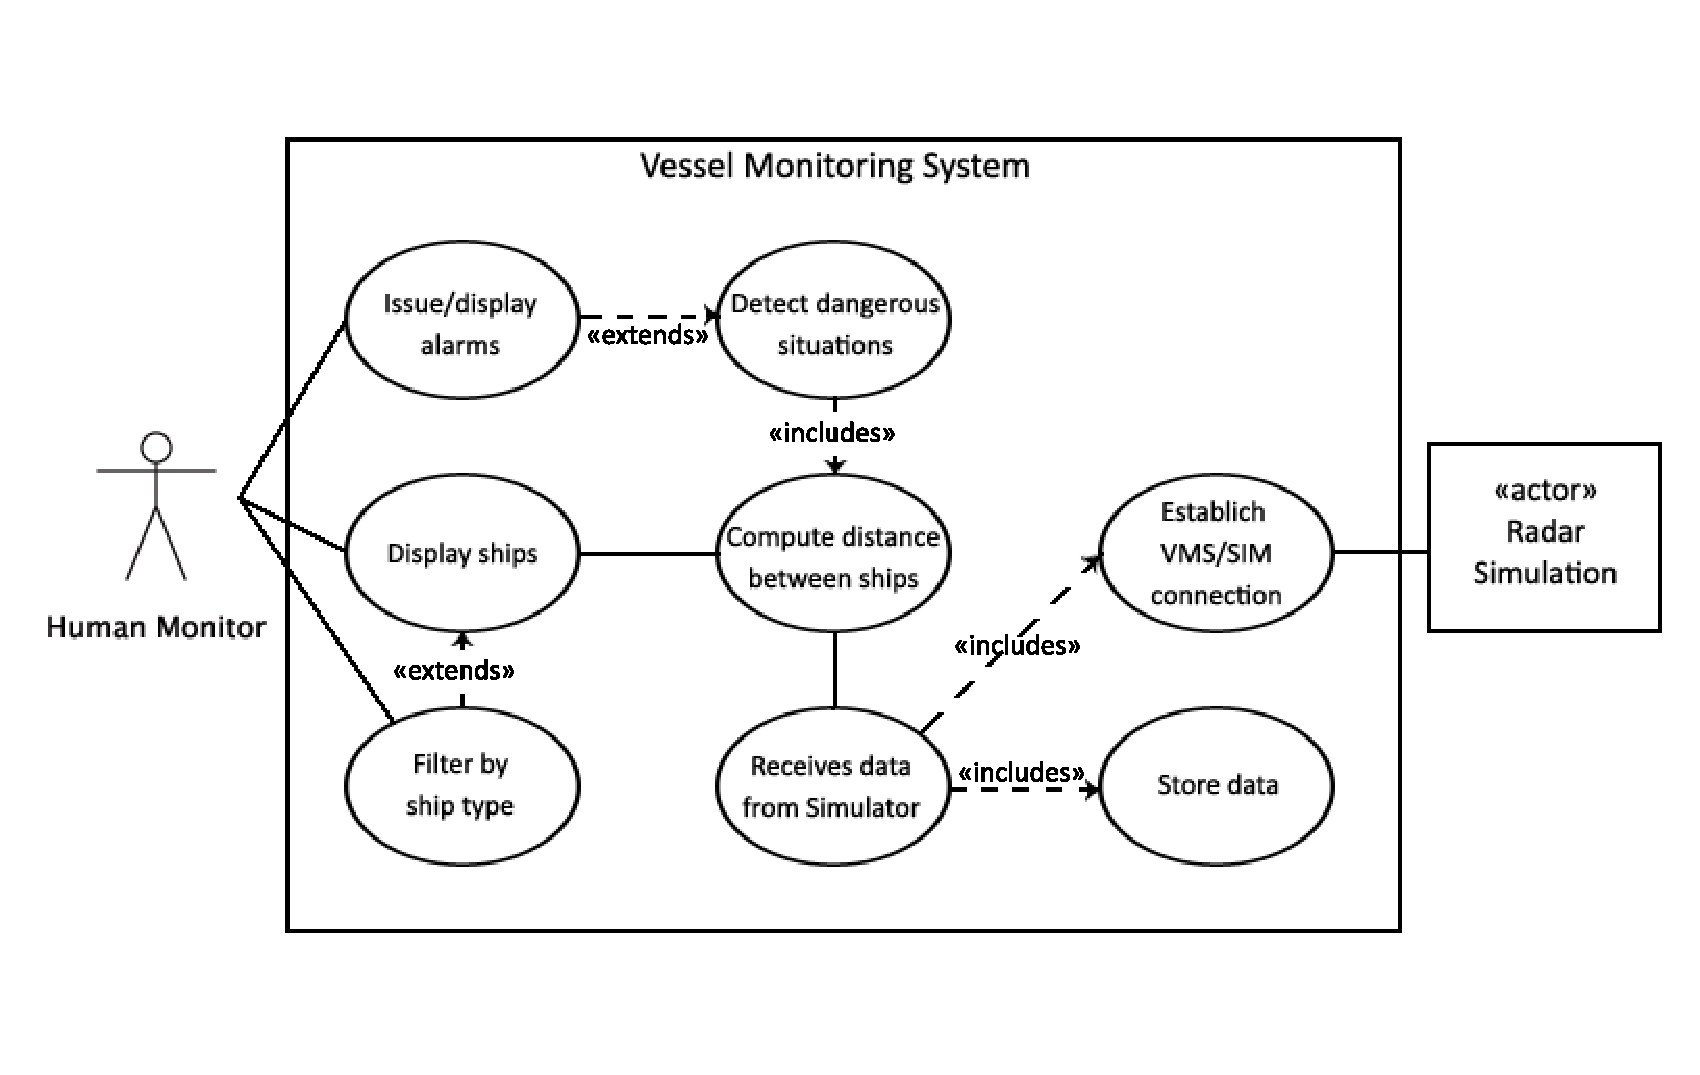
\includegraphics[width=\linewidth]{vmsdiagram.eps}
\end{figure}

\subsubsection{Use Case 1} \label{uc:1}

\noindent
{\bf Name}\\
Vessel Monitoring System - Normal State

\noindent
{\bf Summary}\\
The Vessel Monitoring System is used to show the location of various vessels on a map. This Use Case scenario explains what happens
when the Vessel Monitoring System is operation normaly without any alert or problems.

\noindent
{\bf Actors}\\
User, Monitoring System and Radar Simulation.

\noindent
{\bf Precondition}\\
A new ship is ready to send data from the Radar Simulation to the Monitoring System.

\noindent
{\bf Main Scenario}\\
\vspace*{-0.2in}
\begin{enumerate}
\item User open the monitoring system program to check vessel locations.
\item Monitoring System establish a connection with the Radar Simulation.
\item Radar Simulation sends new information to Vessel Monitoring System.
\item Vessel Monitoring System obtains the new information from the Radar Simulation and stores the data.
\item Vessel Monitoring System updates the information shown on the User's screen.
\item User can filter through different types of vessels and select the ones they want to display.
\item Monitoring system displays only the vessels choosen by the user.
\item User closes the Vessel Monitoring System program.
\end{enumerate}

\noindent
{\bf Exceptions}\\
Vessel Monitoring System is not receiving the data from the Radar Simulation and cannot display the vessels.

\noindent
{\bf Postcondition}\\
\vspace*{-0.2in}
\begin{enumerate}
\item The Vessel Monitoring System receives and store the data correctly and the ship's position is updated on the screen.
\item The System is now waiting for new data to arrive.
\end{enumerate}

\noindent
{\bf Priority}\\
1

\noindent
{\bf Traces to Test Cases}\\
Add when test cases done.

\subsubsection{Use Case 2} \label{uc:2}

\noindent
{\bf Name}\\
Vessel Monitoring System - Alert State

\noindent
{\bf Summary}\\
The Vessel Monitoring System is used to show the location of various vessels on a map. This Use Case scenario explains what happens
when the Vessel Monitoring System needs to display an alert because the distance between two or more vessels is too short.

\noindent
{\bf Actors}\\
User, Monitoring System and Radar Simulation.

\noindent
{\bf Precondition}\\
A new ship is ready to send data from the Radar Simulation to the Monitoring System and two ships are too close to each other.

\noindent
{\bf Main Scenario}\\
\vspace*{-0.2in}
\begin{enumerate}
\item User open the monitoring system program to check vessel locations.
\item Monitoring System establish a connection with the Radar Simulation.
\item Radar Simulation sends new information to Vessel Monitoring System.
\item Vessel Monitoring System obtains the new information from the Radar Simulation and stores the data.
\item Vessel Monitoring System updates the information shown on the User's screen.
\item Vessel Monitoring System detects that two ships are near each other and displays an alert.
\item User closes the Vessel Monitoring System program.
\end{enumerate}

\noindent
{\bf Exceptions}\\
Vessel Monitoring System is not receiving the data from the Radar Simulation and cannot display the vessels.\\
The vessels are not near each other enough to create an alert.

\noindent
{\bf Postcondition}\\
\vspace*{-0.2in}
\begin{enumerate}
\item The Vessel Monitoring System receives and store the data correctly and the ship's position is updated on the screen.
\item The Vessel Monitoring System hides the warning once the threat is gone.
\item The System is now waiting for new data to arrive.
\end{enumerate}

\noindent
{\bf Priority}\\
1

\noindent
{\bf Traces to Test Cases}\\
Add when test cases done.

\end{document}
